\chapter{Introduction}

Prior to the advent of computers, data processing was predominantly a manual task that involved a considerable amount of time, effort, and the potential for human errors. Organizations, particularly businesses, faced challenges in handling large volumes of data efficiently and accurately. This led to a demand for automated systems that could streamline data processing and eliminate the limitations associated with manual methods. The development of computers offered a solution to these challenges by providing a means to automate data-related tasks. It allowed storing and processing larger amounts of data than ever before.
\par
A couple of decades later, data is one of the most important resources for many companies. It helps them run their business more efficiently and make better business decisions. Data pipelines have emerged as crucial components in modern business infrastructures. In general, a data pipeline refers to a system or framework that facilitates the flow of data from various sources to its destination, typically for processing, analysis, storage, or visualization. It is a series of interconnected steps or processes that enable the extraction, transformation, and loading (ETL) of data, ensuring that it moves efficiently and reliably through the pipeline.
\par
A simple example of a data pipeline might be saving contents of a form filled by a customer on a web page to a database. Another, a more complex one might be a preparation of marketing success report where data from recent sales stored in an accounting system are correlated with a list of latest advertising campaign exported from a marketing tool and compared with customer satisfaction form result which might be stored in a database as in the previous example. It is easy to see that these pipelines might become long and complex and that they can be chained one after the other. Less obvious is that they are often facilitated by multiple systems. It would be easier to manage if they were facilitated by one, but there are often reasons why that is not possible. There is no universal tool, each serves a different purpose. A database is great for storing data and fast queries over large data sets, ETL tools are good in data transformations, reporting tools are great for data visualization and analytic and machine learning tools are essential for data science. There might even be a legacy system that cannot be easily migrated to a different platform. They all compose a data environment which serves one purpose - to run business more effectively and make good business decisions.
\par
As the Greek philosopher Heraclitus said, \textit{the only constant in life is change}. This statement is fitting for data environments, because they always change. A new column is added to a schema, two are removed, a new process is introduced or an existing one needs to be modified or fixed etc. A change may span across multiple systems or a modification in one system may influence other systems that depend on it. Planning it can become a nightmare, because even if there is a support for impact analysis in each system, there is none environment-wide and has to be prepared manually. That is why additional processes were developed that help making changes with predictable outputs, without causing errors and that ensure data correctness afterwards. One of such processes is called \textit{data lineage}. 
%% TODO: add also a note about data governance/data quality and migrations

\section{Data lineage}

Data lineage is a process of mapping and visualizing data flows within a data environment. It tracks data as they flow from various sources to their destinations and their transformations with aim to help manage and develop data environments. It provides a comprehensive understanding of how data is acquired, manipulated, and utilized within an organization. Data lineage offers several benefits to businesses and data professionals. Firstly, it enhances data governance and regulatory compliance by ensuring transparency and traceability of data. It enables organizations to meet the requirements of various regulations such as GDPR or CCPA. Secondly, data lineage improves data quality and accuracy by identifying data inconsistencies, errors, or gaps in the data flow. This helps in identifying and rectifying issues promptly, leading to reliable and trustworthy data insights. Additionally, data lineage facilitates data discovery, data integration, and data analytics processes, as it provides a clear understanding of data origins and transformations. It enables faster troubleshooting and root cause analysis, reducing the time and effort required for resolving data-related issues. Overall, data lineage plays a crucial role in maximizing the value of data assets and ensuring data integrity, trust, and accountability within an organization.
\par
Data lineage can be obtained by hand from teams of analysts that map data environments or, more recently, using one of the automated systems that are being developed. Manual data lineage analysis is time- and labor-intensive, so developing automated solutions can provide more up-to-date results and decrease costs.
\par
\textit{Manta Flow} is an automated data lineage platform. It can analyze complex data environments consisting of various databases, data integration and reporting tools and applications in Java, C\# or Python. Using metadata extracted from each connection to a system, Manta Flow computes data lineage graphs where vertices represent data sources and directed edges represent data flows between them. At first, a graph is constructed and stored for each individual connection. When the data lineage is visualized, the graphs are retrieved from the repository and combined together to show a graph of the entire environment.

\begin{figure}[ht]\centering
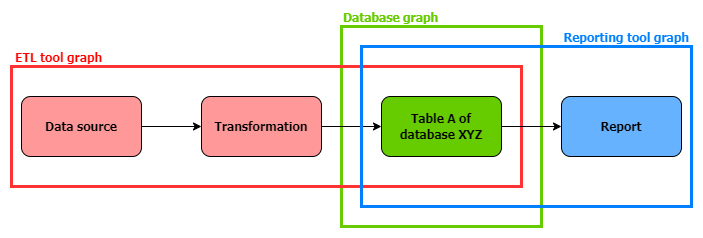
\includegraphics[width=1.0\textwidth]{img/graph_example.png}
\caption{An example of combined data lineage graph}
\label{figGraphExample}
\end{figure}  

\par
To illustrate this with an example, let us have an ETL tool which contains a pipeline writing data into table A of database XYZ and a reporting tool which visualizes data from this table in a report. The analysis would produce three graphs:
\begin{itemize}
    \item an ETL tool graph which contains data pipeline data flow ending with a write to table A,
    \item a database XYZ graph which represents table A and its columns,
    \item a reporting tool graph that contains data read from table A into a report. 
\end{itemize}
These graphs would be visualized as one unified data lineage, as seen in figure~\ref{figGraphExample}.

\section{Embedded code}
Various data processing, management and analytic tools have been developed to allow their users to extract important pieces of information from the vast amounts of data they collect. These tools often provide graphical interface for creating data pipelines consisting of commonly used data sources and transformations. Using such tool opens data pipeline management to a wider, less technically proficient audience, so business-oriented employees can be involved more closely in the development. An example of such tool may be AWS Glue platform where users may define their ETL pipeline using graphical interface with multiple data sources, transformations and joins without having to write a single line of code. However, data can be very dynamic and different and it would be difficult to define every possible data transformation that the users might require. In such cases these tools often allow extending the pipeline with embedded code.
\par
Embedded code is a piece of code provided by a user that is safely executed in the context of the tool and can perform (almost) any desired task. It is often a function or a script. Popular examples of tools that support embedded code include already-mentioned AWS Glue, but also Databricks platform, Snowflake data cloud or SQL Server Integration Services (SSIS) etc. Programming languages used in embedded code often include the popular and well-known ones such as Python, Java, Scala or C\#.
\par
Embedded code can be used to perform a data transformation in an ETL pipeline that is not included in the toolbox, read data from an unsupported data source or to create a user-defined database function that cannot be written efficiently in SQL.
\par
Data flow analysis of embedded code is a crucial missing link in Manta Flow. It can analyze both data pipeline metadata and standalone Python, Java or C\# applications, but there is no support when such a piece of code is a part of the pipeline. Missing embedded code data lineage causes logical gaps in the holistic data lineage and decreases its usability, because these gaps have to be filled in by hand. Following the recent surge in demand for data science and machine learning solutions where especially Python is the programming language of choice, the number of enterprise data environments which contain embedded code has also risen significantly. This drives the market demand for data lineage solutions that can cope with it. As there are currently no solutions that can reliably provide it, extending current capabilities of Manta Flow in data flow analysis of applications to embedded code shall provide it a significant competitive advantage.

\section{AWS Glue}

AWS Glue is a serverless data integration service that makes it easier to discover, prepare, move, and integrate data from multiple sources for analytics, machine learning and application development. It performs data processing on Apache Spark engine in a cloud environment. Data pipelines are defined using embedded code, supported programming languages are Python and Scala. They can also be created from the GUI, where the tool generates the corresponding pipeline code. This service is especially convenient for companies that already use other AWS services as it can efficiently use such resources.
\par
AWS Glue has been on top of the list of technologies to be supported by Manta Flow based on customer enquiries. There is currently very limited support for automated AWS Glue data lineage on the market, so having it provides a competitive advantage. As the pipelines consist of embedded code, analyzing it is the best, although a very difficult way to extract data lineage information. However, Manta Flow can already analyze Python and Bytecode (Scala is compiled into Bytecode) applications. Extending the analysis support with embedded code is therefore a direct prerequisite for a successful AWS Glue data lineage analysis.

\section{Goals}

The goal of this thesis is to design a data lineage analysis service for embedded code in Manta Flow that will enable integration of data lineage graph from data processing and analytic tools with the data lineage graph derived from the embedded code.
\par
One of the main tasks is to create a solid design of the service that should be easily extendable with support for new tools and their embedded code in the future. Benefits and usefulness of this design will be then demonstrated on a prototype implementation of the service for AWS Glue and the embedded code written in Python.
\par
Other specific tasks include a proof-of-concept implementation of a metadata extractor for AWS Glue and modifications to the existing Python scanner. A very important aspect of the service is high performance, because it will be called many times during a run of the Manta Flow analysis platform, specifically every time the analysis processes a statement that executes a piece of embedded code.

\section{Outline}

This thesis is split into several chapters. In introduction we briefly describe the motivation and the goal of the thesis. In the second chapter we describe important aspects of MANTA Flow platform with which the service developed in this thesis is integrated. Chapter 3 is dedicated to a detailed problem analysis and we formulate our requirements there. Chapter 4 delves into design and implementation of embedded code service and changes that were made to Python scanner. In chapter 5 we take a look at the design and proof-of-concept implementation of AWS Glue scanner, which uses embedded code service for data flow analysis of embedded Python code. In chapter 6 we demonstrate the functionality of implemented features on several examples and discuss the limitations of the implementation. Finally, in conclusion we sum up what we achieved in this work and how we did it.